\documentclass[12pt,a4paper]{article}
\usepackage[utf8]{inputenc}
\usepackage[english,finnish]{babel}
\usepackage{amsmath}
\usepackage{amsfonts}
\usepackage{amssymb}
\usepackage{graphicx}
\usepackage[left=2cm,right=2cm,top=2cm,bottom=2cm]{geometry}
\usepackage{hyperref}

\title{Projektinhallintajärjestelmä\\Suunnitteludokumentti}

\author{Markus Korpinen}

\begin{document}
\maketitle
\section*{Johdanto}
Toteutetaan projektinhallintajärjestelmä, jonka avulla voidaan seurata eri projektien etenemistä. Käyttäjät voivat kirjautumisen jälkeen luoda omia projekteja ja jakaa niitä muiden käyttäjien kanssa. Projektien alle voidaan asettaa  tehtäviä eri prioriteeteillä ja aikatauluilla. Projektinhallintajärjestelmä toteutetaan käyttäen Ruby-kieltä ja MVC-malliin pohjautuvaa Ruby on Rails -ohjelmistokehystä. Tietokantannaksi valitaan PostgreSQL ja Web-palvelimeksi WebRICK. Versionhallintana käytetään gitiä ja ohjelmisto julkaistaan Heroku.com palvelussa.

\section*{Yleiskuva järjestelmästä}
\subsection*{Käyttäjäryhmät}
Käyttäjäryhmien oikeudet kasvavat alhaalta ylös, ts. kaikkien alempana olevien käyttäjäryhmien
oikeudet ovat myös ylempänä olevilla.
\subsubsection*{Luoja}
Luo uuden projektin ja on siten samalla automaattisesti myös projektin hallinnoija. Erona projektin
hallinnoijaan on se, että vain luoja voi poistaa projektin. Kuka tahansa rekisteröitynyt käyttäjä voi luoda
uuden projektin ja kutsua siihen muita käyttäjiä.
\subsubsection*{Hallinnoija}
Hallinnoijalla on kaikki oikeudet muokata projektia ja projektin tehtäviä, sekä luoda projektiin uusia
tehtäviä. Hallinnoijat voivat osoittaa tehtäviä projektin jäsenten vastuulle. Hallinnoijat voivat myös
kutsua muita käyttäjiä projektin jäseniksi.
\subsubsection*{Jäsen}
Projektin jäsen voi lunastaa itselleen projektin tehtäviä joko valitsemalla niitä listasta tai
hyväksymällä hallinnoijien heille osoittamia tehtäviä, sekä merkitä tehtäviä tehdyiksi.
\subsubsection*{Rekisteröitynyt}
Rekisteröitynyt käyttäjä voi luoda järjestelmään uusia, joko julkisia tai yksityisiä projekteja ja lähettää
pyynnön saada liittyä olemassaolevan projektin jäseneksi. Luomalla uuden projektin hänestä tulee
kyseisen projektin luoja.
\subsubsection*{Vierailija}
Vierailija voi selata järjestelmän julkisia projekteja ja rekisteröityä järjestelmän käyttäjäksi.

\section*{Käyttötapaukset}

\subsubsection*{Rekisteröityminen}
Vierailijat voivat rekisteröityä projektinhallintajärjestelmän käyttäjiksi.

\subsubsection*{Projektien selaaminen}
Rekisteröityneet käyttäjät voivat selata kaikkia projekteja ja vierailijat voivat selata vain julkisia projekteja.

\subsubsection*{Projektin lisääminen}
Rekisteröitynyt käyttäjä voi perustaa projekteja antamalla riittävän määrän tietoja mm. projektin
tyypistä ja näkyvyydestä (julkinen tai yksityinen), jonka jälkeen hänestä tulee projektin luoja.

\subsubsection*{Projektin poistaminen}
Projektin luoja voi halutessaan poistaa projektin, jolloin kaikki projektiin liittyvä data samalla
tuhoutuu.

\subsubsection*{Tehtävien selaaminen}
Projektiin jäseniksi lisätyt, ja julkisten projektien tapauksessa myös kaikki järjestelmän käyttäjät
voivat selata projektin tehtäväluetteloa, jossa näkyvät kaikki projektiin listatut tehtävät ja niiden tiedot.
Korkeamman prioriteetin omaavat tehtävät näkyvät ylempänä, mutta projektin jäsenet voivat järjestellä
tehtäviä myös nimen tai päivämäärän mukaan. Oletusarvoisesti tehtävälistassa näkyvät kaikki vapaat, eli
lunastamatta olevat tehtävät, mutta projektin jäsenet voivat valita näytettäväksi myös tehtävät jotka on
jo lunastettu tai tehtävät jotka on jo suoritettu.

\subsubsection*{Tehtävän lisääminen projektiin}
Projektin hallinnoijat voivat luoda uusia tehtäviä projektiin kirjoittamalla tehtäväkuvauksen, tehtävän
prioriteetin, tehtävän aikataulun ja muita tarvittavia tietoja, jonka jälkeen tehtävä ilmestyy projektin
tehtäväluetteloon.

\subsubsection*{Tehtävän poistaminen projektista}
Projektin hallinnoijat voivat poistaa tavallisia jäseniä projektista, jolloin näiden mahdolliset lunastetut
tehtävät kommentteineen palaavat avoimiksi tehtäväluetteloon. Hallinnoijia voi poistaa projektista
ainoastaan projektin luoja.

\subsubsection*{Tehtävän lunastaminen}
Projektin jäsenet voivat lunastaa tehtäviä itselleen tai hyväksyä hallinnoijien heille osoittamia
tehtäviä, jolloin kyseinen tehtävä siirtyy tehtäväluettelosta jäsenen omaan tehtävälistaan. Käyttäjät voivat
merkitä edistymistään tehtävässä kommenteilla.

\subsubsection*{Tehtävän suorittaminen}
Tehtävän tultua tehdyksi, käyttäjä merkitsee sen suoritetuksi ja kirjoittaa tarvittaessa tarkentavan
kommentin suorituksesta, jolloin se siirtyy suoritettujen tehtävien luetteloon. Samalla hän kirjaa
ajankäyttönsä tunteina.

\subsubsection*{Tehtävästä luopuminen}
Tehtävän luonut projektin hallinnoija tai projektin luoja voi poistaa tehtävän projektista, jolloin
kaikki tehtävään liittyvä data samalla tuhoutuu ja mahdollisesti lunastettu tehtävä poistuu sen
lunastaneen omasta tehtävälistasta.

\section*{Järjestelmän tietosisältö}
\begin{figure}[h!]
	\centering
	\caption{Luokkakaavio järjestelmän tietosisällöstä,}
	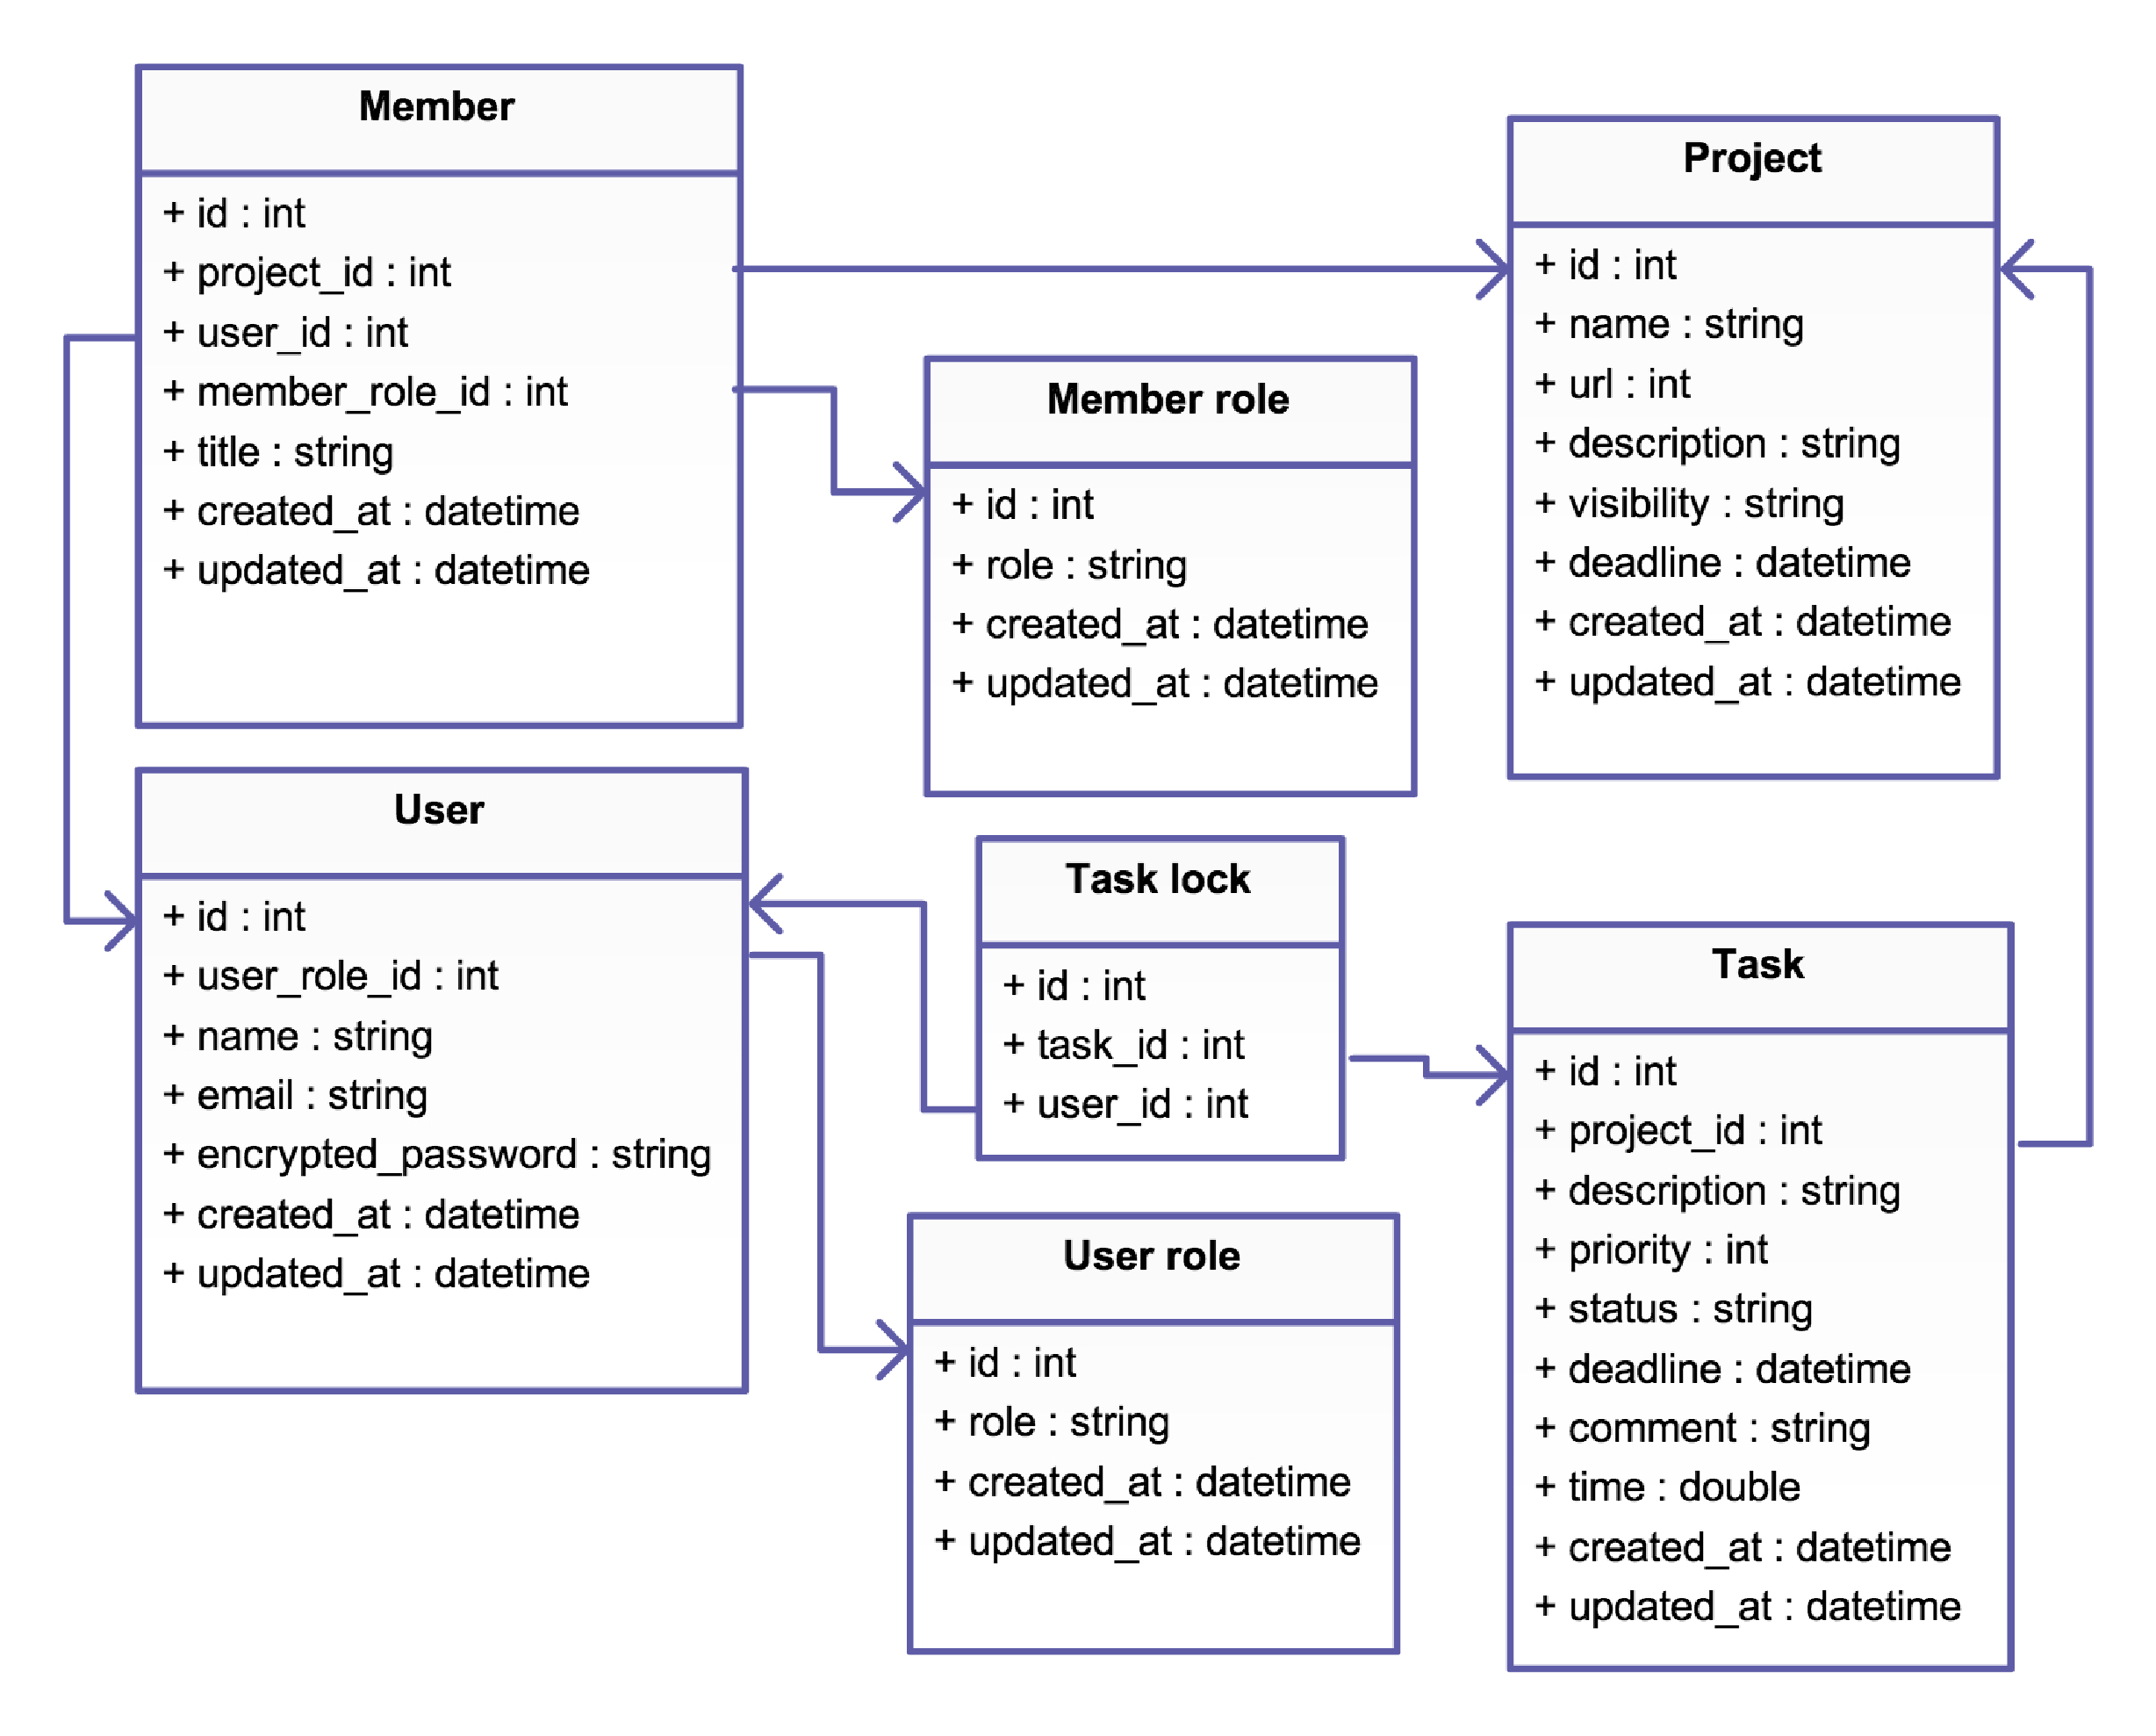
\includegraphics[width=0.9\textwidth]{luokkakaavio.pdf}
\end{figure}

\subsection*{Käyttäjä (user)}
Id, käyttäjäroolin id, nimi, sähköposti, salasanan suola, salasana kryptatussa muodossaan, luontiaika,
muokkausaika.
Käyttäjärooli tarkoittaa järjestelmän käyttäjän roolia järjestelmässä, ei siis projekteissa.
\subsection*{Käyttäjärooli (user role)}
Id, roolin nimi, luontiaika, muokkausaika
Rooleja ovat esimerkiksi ”käyttäjä” tai ”järjestelmän admin”.
\subsection*{Projekti (project)}
Id, nimi, web-sivun url, kuvaus, näkyvyys, deadline, luontiaika, muokkausaika.
Projektin kuvaus on vapaa tekstikenttä, näkyvyys tarkoittaa joko yksityistä tai julkista ja deadline
päivämäärä johon mennessä projektin on oltava valmis.
\subsection*{Tehtävä (task)}
Id, projektin id, kuvaus, prioriteetti, tehtävän status, deadline, suorituskommentti, ajankäyttö,
luontiaika, muokkausaika.
Tehtävän status voi olla esim. ”suorittamatta”, ”suorituksessa”, ”suoritettu” tai ”hylätty”.
Suoritettuun tehtävään liittyy suorituskommentti, jonka projektin jäsen kirjoittaa suoritettuaan
tehtävän. Jäsen kirjaa myös tehtävän ajankäyttönsä tunteina.
\subsection*{Jäsen (member)}
Id, projektin id, käyttäjän id, jäsenroolin id, nimitys, luontiaika, muokkausaika.
Jäsenellä voi jäsenroolin lisäksi olla nimitys, esim. ”projektipäällikkö”, ”ohjelmoija”, ”juhlamestari”,
jne.
\subsection*{Jäsenrooli (member role)}
Id, rooli, luontiaika, muokkausaika.
Käyttäjärooleilla tarkoitetaan projektissa olevien jäsenten rooleja: ”jäsen”, ”hallinnoija” ja ”luoja”.
\subsection*{Tehtävän lukitus (task lock)}
Id, tehtävän id, osoitetun käyttäjän id, osoittavan käyttäjän id, luontiaika, muokkausaika.
Hallinnoijan osoittaessa tehtävän projektin jäsenelle tallentuu osoittavan käyttäjän id ja sen jäsenen
id jolle tehtävä osoitetaan erikseen. Jäsenen lunastaessa tehtävän, molempiin näihin kenttiin tulee hänen
id:nsä.

\end{document}